\chapter{Lecture 2: ....}\label{lec:2}
\section{Fieldbus systems OSI Layers used}

\begin{itemize}
\item Mostly layers 3 to 6 are nonexistent
\begin{itemize}
\item Efficient, fast data processing
\item No routing
\item No fragmentation
\end{itemize}
\end{itemize}

\textbf{But a fieldbus is different.}

In a bus system:

\begin{itemize}
\item Everything is inside a closed system (e.g., a car)
\item All nodes share the same physical network
\item There is no concept of ``routing between networks''
\item There is no need for end-to-end transport across multiple hops
\end{itemize}

\textbf{So yes:}

\begin{itemize}
\item \checkmark \ No Layer 3 (Network layer)
\begin{itemize}
\item No routing between networks
\item No IP-style addressing needed
\item Every node already ``hears'' the same medium
\end{itemize}

\item \checkmark \ No Layer 4 (Transport layer)
\begin{itemize}
\item No TCP-like connection management
\item Reliability is handled differently (or not needed at that level)
\item Messages are small and time-critical
\end{itemize}

\item \checkmark \ No Layers 5--6
\begin{itemize}
\item No session negotiation between applications
\item No complex data translation layer needed
\item Encoding is usually fixed and defined by the protocol/application design
\end{itemize}
\end{itemize}

\subsection{So what is left?}

Most fieldbus systems only implement:

\begin{itemize}
\item Layers 1--2 (always)
\begin{itemize}
\item Physical layer (wires, voltage, timing)
\item Data link layer (frames, arbitration, error detection)
\end{itemize}

\item Sometimes Layer 7
\begin{itemize}
\item Application layer (what messages mean)
\item Example: ``engine RPM = 3000''
\item But no deeper networking stack underneath
\end{itemize}
\end{itemize}

\section{Controller Area Network (CAN) at a glance}

\begin{itemize}
    \item \textbf{Number of nodes}
    \begin{itemize}
        \item Unlimited (dependent on physical layer)
    \end{itemize}

    \item \textbf{Topology}
    \begin{itemize}
        \item Line
        \item Star
    \end{itemize}

    \item \textbf{Length of bus lines (dependent on transfer rate)}
    \begin{itemize}
        \item 40 m at 1 Mbit/s (specified)
        \item 620 m at 100 kbit/s
        \item 10 km at 5 kbit/s
    \end{itemize}

    \item \textbf{Number of message identifiers}
    \begin{itemize}
        \item $2^{11}$ (standard frame)
        \item $2^{29}$ (extended frame)
    \end{itemize}

    \item \textbf{Data bytes per message}
    \begin{itemize}
        \item 0--8 bytes
    \end{itemize}

    \item \textbf{Bus access}
    \begin{itemize}
        \item CSMA/CD with AMP (Carrier Sense Multiple Access / Collision Detection with Arbitration on Message Priority)
        \item Controlled by message priority
        \item Non-destructive bit-wise arbitration
    \end{itemize}

    \item \textbf{Bus throughput}
    \begin{itemize}
        \item Max. 1 Mbit/s (total)
        \item Max. 577 kbit/s (useful information / payload)
    \end{itemize}

    \item \textbf{Real-time capability}
    \begin{itemize}
        \item Guaranteed latency for high-priority messages
        \item $< 134\,\mu s$ at 1 Mbit/s
    \end{itemize}

    \item \textbf{Reliability / Safety}
    \begin{itemize}
        \item Acknowledgment of messages
        \item Error detection, handling, and fault confinement
    \end{itemize}

\end{itemize}
\section{CAN bus architecture and L1}
\begin{figure}[H]
    \centering
    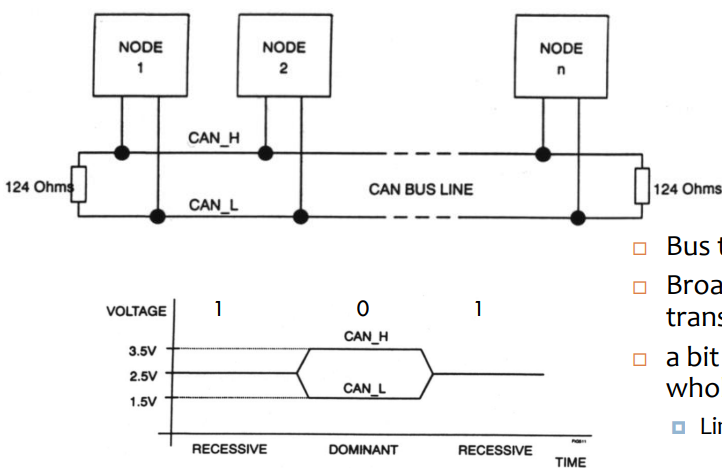
\includegraphics[width=0.8\linewidth]{figures/Lecture2/CanbusBus.png}
    \label{fig:placeholder}
\end{figure}
\begin{itemize}

\item \textbf{2. Broadcast transmissions}

When one node sends a message:
\begin{itemize}
    \item It is transmitted onto the entire bus
    \item Every node receives it
    \item Nodes decide themselves whether to use it or ignore it
\end{itemize}

So there is no direct addressing like ``send only to ECU X''.

It is more like:
\begin{quote}
``Everyone hears everything, but only some care.''
\end{quote}

\item \textbf{3. A bit must ``fill'' whole bus}

This is the key physical-layer idea.

When a node sends a bit (0 or 1):
\begin{itemize}
    \item That electrical signal must propagate along the entire cable
    \item Every node must see the same bit value at (almost) the same time
\end{itemize}

So the system assumes:
\begin{quote}
The signal is ``present everywhere on the bus'' before the bit time ends.
\end{quote}

\item \textbf{4. Limits cable length}

This is the consequence of the previous point.

Signals travel at a finite speed (speed of electricity in the cable). So:
\begin{itemize}
    \item If the cable is too long
    \item The signal takes too long to reach the far end
    \item Different nodes may ``see different bit values at the same time''
\end{itemize}

That breaks correctness (especially arbitration in CAN).

So:
\begin{quote}
Longer cable $\rightarrow$ slower propagation $\rightarrow$ lower maximum bitrate
\end{quote}

That is why CAN has trade-offs like:
\begin{itemize}
    \item Short cable $\rightarrow$ high speed (1 Mbit/s)
    \item Long cable $\rightarrow$ low speed (e.g., 5 kbit/s over kilometers)
\end{itemize}

\end{itemize}

\section{CanBus Bit timing}

\begin{itemize}

\item \textbf{1. Why bit timing is needed}

On a CAN bus:
\begin{itemize}
    \item Many ECUs transmit on the same wire
    \item There is no central clock
    \item Yet everyone must agree whether the current bit is 0 or 1
\end{itemize}

So every node must stay synchronized while ``listening'' to the bus.

\item \textbf{2. Bit synchronization using edges}

CAN does not use a shared clock. Instead it uses:
\begin{quote}
signal transitions (edges) to resynchronize timing
\end{quote}

What that means:
\begin{itemize}
    \item If bits keep changing (0 $\rightarrow$ 1 or 1 $\rightarrow$ 0), nodes can re-align their internal clocks
    \item Each node slightly adjusts its timing based on when it sees a transition
\end{itemize}

Problem:
\begin{itemize}
    \item If a long sequence has no changes (e.g. 11111111)
    \item Nodes can drift apart in timing
    \item They may disagree on bit boundaries
\end{itemize}

Solution:
\begin{quote}
$\rightarrow$ bit stuffing
\end{quote}

CAN automatically inserts a ``dummy bit'' after a long sequence of identical bits to force transitions.

\item \textbf{3. Bit stuffing idea}

If there are too many identical bits:
\begin{itemize}
    \item The transmitter inserts an opposite bit
    \item Receivers ignore it logically
    \item But use it to re-sync timing
\end{itemize}

So transitions are guaranteed often enough.

\item \textbf{4. Arbitration requirement (very important CAN concept)}

CAN uses:
\begin{itemize}
    \item Dominant bit = 0 (strong signal)
    \item Recessive bit = 1 (weak signal)
\end{itemize}

If two nodes transmit at the same time:
\begin{itemize}
    \item Dominant overwrites recessive
    \item All nodes can see the change immediately
\end{itemize}

So:
\begin{quote}
A node must detect a change (1 $\rightarrow$ 0) before the bit ends
\end{quote}

Otherwise arbitration would fail.

\item \textbf{5. Bit time $\geq 2 \times$ propagation delay}
\begin{figure}[H]
    \centering
    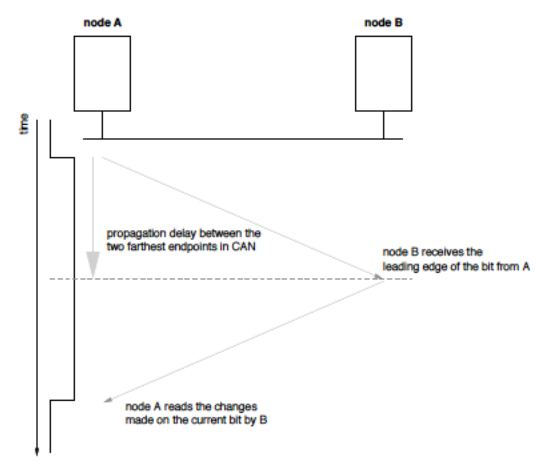
\includegraphics[width=0.8\linewidth]{figures/Lecture2/progationtiming.png}
    \label{fig:placeholder}
\end{figure}
This is a physical constraint.

Signals take time to travel along the cable:
\begin{itemize}
    \item Node A sends a bit
    \item Node B far away receives it slightly later
\end{itemize}
So engineers require:
\[
\text{Bit time} \geq 2 \cdot \text{propagation delay (max distance)}
\]
Why ``2$\times$''?

Because:
\begin{itemize}
    \item Signal must travel from one end to the other
    \item AND the effect of arbitration must travel back
\end{itemize}
So worst-case round-trip delay is considered.
\end{itemize}
\section{CanBus Format}
\begin{figure}[H]
    \centering
    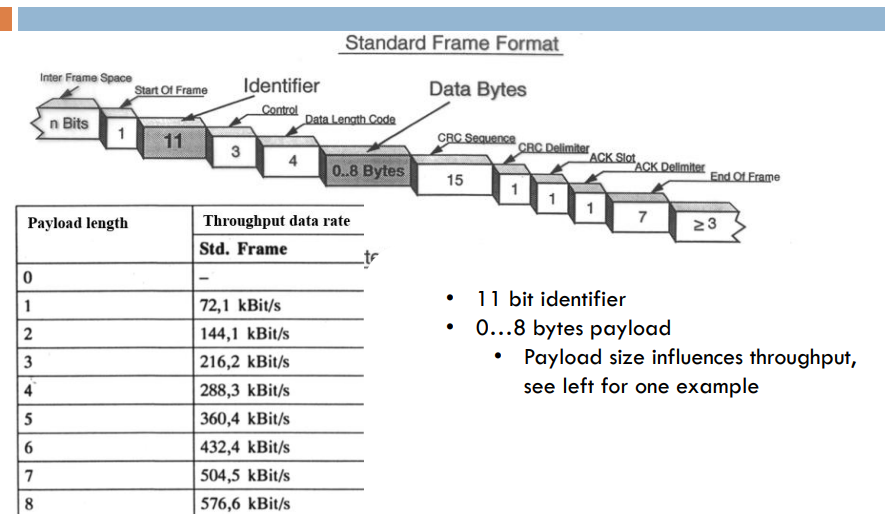
\includegraphics[width=\linewidth]{figures/Lecture2/canbusFormat.png}
    \label{fig:placeholder}
\end{figure}
\textbf{Node:} Number of message identifiers
    \begin{itemize}
        \item $2^{11}$ (standard frame)
        \item $2^{29}$ (extended frame)
    \end{itemize}

\clearpage
\section{CanBus arbitration CAN ID (message identifier)(Not node id)}

\begin{itemize}

\item \textbf{Overwriting in CAN}

CAN uses two bit states:
\begin{itemize}
    \item Dominant = 0 (strong signal)
    \item Recessive = 1 (weak signal)
\end{itemize}

If multiple nodes transmit at the same time:
\begin{itemize}
    \item 0 + 1 $\rightarrow$ bus becomes 0
    \item 1 + 0 $\rightarrow$ bus becomes 0
    \item 1 + 1 $\rightarrow$ bus becomes 1
\end{itemize}

So dominant bits \textbf{overwrite recessive bits} on the bus.

\item \textbf{When a node stops transmitting}

All nodes transmit and listen at the same time.

If a node sends a recessive bit (1) but reads a dominant bit (0):
\begin{itemize}
    \item It immediately knows another node has higher priority
    \item It stops transmitting
\end{itemize}

This prevents data corruption and resolves collisions instantly.

\item \textbf{How priority works (arbitration)}

CAN arbitration is a bit-by-bit competition using the message ID:

\begin{itemize}
    \item Lower binary ID = higher priority
    \item Dominant (0) always wins over recessive (1)
\end{itemize}

Nodes transmit their ID while monitoring the bus:
\begin{itemize}
    \item If a node sends 1 but sees 0, it loses arbitration
    \item It stops immediately
\end{itemize}

\item \textbf{Example}

\begin{center}
\begin{tabular}{l l}
Node A & 0 1 1 ... \\
Node B & 0 0 1 ...
\end{tabular}
\end{center}

Step-by-step:
\begin{itemize}
    \item Bit 1: 0 vs 0 $\rightarrow$ continue
    \item Bit 2: 1 vs 0 $\rightarrow$ bus = 0
    \item Node A sent 1 but sees 0 $\rightarrow$ loses and stops
    \item Node B continues and wins
\end{itemize}

\end{itemize}
\section{Visual representation of arbitration}
\begin{figure}[H]
    \centering
    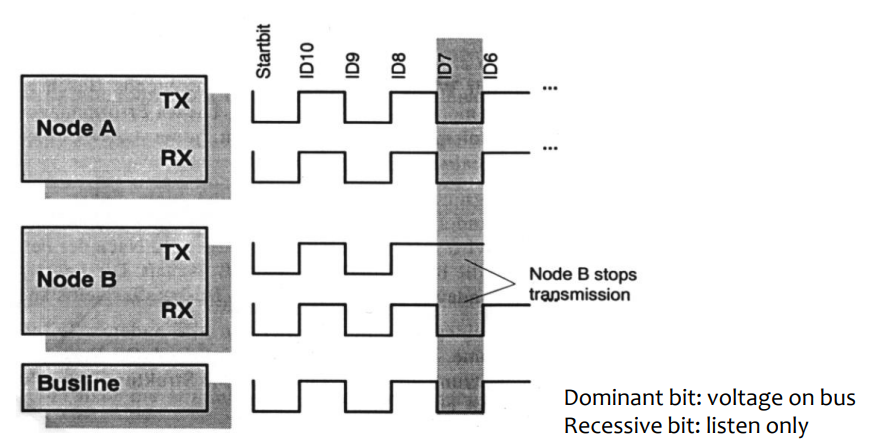
\includegraphics[width=0.8\linewidth]{figures/Lecture2/CANarbitration.png}
    \label{fig:placeholder}
\end{figure}
\begin{mdframed}[backgroundcolor=lightgray, linewidth=0pt, innertopmargin=8pt,
innerbottommargin=8pt]
\textbf{Note (wrong representation of bus in figure):}
RX basically just Busline, and also in reality we would have "Dual-wire bus” / “differential bus"
\begin{itemize}
    \item CAN\_H (CAN High)
    \item CAN\_L (CAN Low)
\end{itemize}
\end{mdframed}

\section{CAN bus advantages}

\begin{itemize}

\item \textbf{Possibility of assigning priority to messages}

CAN uses message IDs to define priority.

\begin{itemize}
    \item Lower ID = higher priority
    \item Important signals (e.g., braking) win access to the bus first
    \item Low-priority data (e.g., infotainment) waits
\end{itemize}

This ensures safety-critical messages are always sent first.

\item \textbf{Guaranteed maximum latency for high-priority messages}

Because of arbitration:

\begin{itemize}
    \item High-priority messages always win bus access
    \item They are never blocked by lower-priority traffic
\end{itemize}

This gives deterministic timing, meaning:
\begin{quote}
You can guarantee worst-case delay for critical signals (e.g., $<134\,\mu s$ at 1 Mbit/s in some systems)
\end{quote}

\item \textbf{Multicast communication with bit-oriented synchronization}

CAN is inherently broadcast-based:

\begin{itemize}
    \item One transmission is received by all nodes
    \item Nodes decide if the message is relevant
\end{itemize}

At the same time:
\begin{itemize}
    \item All nodes stay synchronized using bit timing (edges + stuffing)
\end{itemize}

Result:
\begin{quote}
Efficient ``one-to-many'' communication without needing routing or addressing
\end{quote}

\item \textbf{Error detection}

CAN has strong built-in error handling:

\begin{itemize}
    \item Bit monitoring (detects mismatches while transmitting)
    \item CRC checks (detects data corruption)
    \item Frame format checks
    \item Acknowledgment checking
\end{itemize}

If an error is detected:
\begin{itemize}
    \item The message is automatically retransmitted
    \item Faulty nodes can be isolated (fault confinement)
\end{itemize}

This makes CAN highly reliable in noisy environments like vehicles.

\end{itemize}



\section{CAN configuration complexity and verification}

\subsection*{1. CAN configuration complexity}

Modern \textit{Controller Area Network (CAN)} systems are no longer ``just a bus with a few ECUs''.

Instead, you now have:

\textbf{Hundreds of messages (CAN IDs)}

Each signal in the car becomes a message type:
\begin{itemize}
\item engine speed
\item brake pressure
\item steering angle
\item battery status
\item airbag trigger
\end{itemize}

So complexity grows because many different message types must share one shared communication medium.

\begin{mdframed}[backgroundcolor=lightgray, linewidth=0pt, innertopmargin=8pt,
innerbottommargin=8pt]
\textbf{Multiple buses + gateways}

Modern cars are not one CAN bus. They have:
\begin{itemize}
\item powertrain CAN
\item chassis CAN
\item infotainment CAN
\item safety CAN
\end{itemize}

These are connected via gateways (ECUs that forward messages between buses).

So now you have:
\begin{itemize}
\item multiple networks
\item message routing between them
\item extra delay from buffering/queueing in gateways
\end{itemize}
\end{mdframed}

\textbf{Real-time constraints (e.g. 5 ms deadlines)}

Some signals must arrive very fast:
\begin{itemize}
\item brake $\rightarrow$ actuator must react within milliseconds
\item airbag $\rightarrow$ even faster
\item steering control $\rightarrow$ tightly bounded delay
\end{itemize}

So the requirement becomes:
\begin{quote}
end-to-end latency must be guaranteed
\end{quote}

Not just ``message gets sent'', but:
\begin{quote}
arrives within time limit
\end{quote}

\textbf{Mixed traffic types}

Two traffic styles exist:
\begin{itemize}
\item periodic $\rightarrow$ sent every fixed interval (e.g. every 10 ms)
\item event-based $\rightarrow$ sent only when something happens
\end{itemize}

This creates unpredictability:
\begin{itemize}
\item sometimes the bus is quiet
\item sometimes many events occur at once
\end{itemize}

\textbf{High bus load (50--60\%+)}

CAN is often designed to run ``almost full'' but not overloaded.

Why:
\begin{itemize}
\item efficient usage
\item still some margin for timing guarantees
\end{itemize}

But high load means small timing variations can cause delays.
\begin{mdframed}[backgroundcolor=lightgray, linewidth=0pt, innertopmargin=8pt,
innerbottommargin=8pt]
\textbf{Big idea:}
The system is too complex to assume it works correctly — timing must be verified.
\end{mdframed}
\subsection*{2. Verification of CAN configuration (what this means)}

Now the question becomes:

\begin{quote}
How do we prove that all messages meet their deadlines?
\end{quote}

Again in \textit{Controller Area Network (CAN)} systems.

\textbf{What we are trying to guarantee}

Example requirement:
\begin{itemize}
\item message every 5 ms $\pm$ 10\%
\item at most 3 consecutive deadline misses
\end{itemize}

This means we care about worst-case reliability, not average behavior.

\textbf{Why this is hard}

Delays depend on interacting effects:
\begin{itemize}
\item arbitration (message priority competition)
\item bus load
\item gateway queues
\item mixed periodic/event traffic
\end{itemize}

So timing is not constant — it depends on the full system state.

\textbf{Method 1: Exhaustive worst-case search}
\begin{itemize}
\item simulate all possible situations
\item find worst-case delay
\end{itemize}

Problem:
\begin{itemize}
\item number of combinations explodes
\item infeasible for large systems
\end{itemize}

Works only for small systems.

\textbf{Method 2: Network calculus}
\begin{itemize}
\item mathematical modelling of traffic
\item computes worst-case delays
\item includes bus speed, priorities, and queueing in gateways
\end{itemize}

Provides formal guarantees.

\textbf{Method 3: Simulation}
\begin{itemize}
\item simulate realistic scenarios
\item observe typical behaviour
\end{itemize}

Good for average performance and debugging, but:
\begin{quote}
no guarantee that worst-case is observed
\end{quote}
\begin{mdframed}[backgroundcolor=lightgray, linewidth=0pt, innertopmargin=8pt,
innerbottommargin=8pt]
\subsection*{3. One combined intuition}

Modern CAN design problem:

\begin{quote}
We have many message types competing for a shared real-time bus, sometimes across multiple networks, and we must guarantee every critical message arrives in time.
\end{quote}

Therefore engineers must:
\begin{itemize}
\item design message priorities (CAN IDs)
\item control bus load
\item analyse worst-case delays
\item verify timing mathematically
\end{itemize}
\end{mdframed}

\clearpage


\section{FlexRay main features (explained simply)}
\todo{Revised and make sure understand comparassion between the two}
\textit{FlexRay} is designed as a deterministic and high-speed alternative to \textit{CAN}, mainly for safety-critical automotive systems.

\begin{itemize}

\item \textbf{1. High data rate (up to 10 Mbit/s)}

\begin{itemize}
    \item Much faster than CAN (typically up to 1 Mbit/s)
    \item Suitable for high-bandwidth signals (e.g. steering systems, sensors, cameras, control data)
\end{itemize}

\item \textbf{2. Time-triggered communication}

Two communication modes:

\begin{itemize}
    \item \textbf{Time-triggered (scheduled)} $\rightarrow$ fixed time slots (fully deterministic)
    \item \textbf{Event-triggered} $\rightarrow$ similar to CAN (send when needed)
\end{itemize}

\begin{quote}
This hybrid design makes the system both predictable and flexible.
\end{quote}

\item \textbf{3. Deterministic behavior}

Main improvement over \textit{Controller Area Network (CAN)}:

\begin{itemize}
    \item In CAN: delays depend on arbitration and bus load
    \item In FlexRay: transmission times are pre-scheduled
\end{itemize}

\begin{quote}
Message delays are bounded and fully predictable.
\end{quote}

No arbitration-induced delay variation and no unexpected timing jitter under load.

\item \textbf{4. Redundancy (dual-channel communication)}

FlexRay uses two independent channels:

\begin{itemize}
    \item Channel A
    \item Channel B
\end{itemize}

Messages can be transmitted on both channels.

\begin{quote}
If one channel fails, the other still ensures communication.
\end{quote}

This significantly improves system reliability compared to CAN.

\item \textbf{5. Fault tolerance (comparison with CAN)}

\textbf{In CAN:}
\begin{itemize}
    \item Error detection (CRC, bit monitoring, frame checks)
    \item Fault confinement (nodes can disconnect themselves if faulty)
    \item Automatic retransmission of corrupted messages
\end{itemize}

\textbf{In FlexRay:}
\begin{itemize}
    \item All CAN-like error detection mechanisms
    \item Plus stronger system-level fault tolerance:
    \begin{itemize}
        \item clock synchronization between nodes
        \item redundant communication paths
        \item dual-channel operation
    \end{itemize}
\end{itemize}

\begin{quote}
FlexRay not only detects errors like CAN, but is also designed to continue correct operation under system-level faults.
\end{quote}

\end{itemize}



\section{Network Topologies (Flexray)}
\begin{figure}[H]
    \centering
    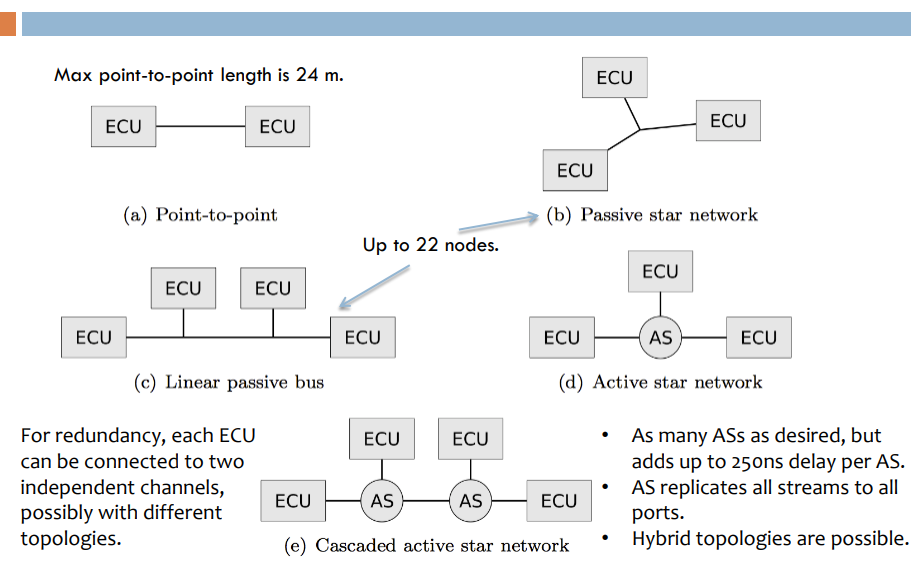
\includegraphics[width=\linewidth]{figures/Lecture2/flexraytoplogy.png}
    \caption{Caption}
    \label{fig:placeholder}
\end{figure}
\begin{enumerate}[label=(\alph*)]


\item \textbf{Passive Star}
\begin{itemize}
    \item Multiple ECUs connected to a central passive junction.
    \item The center has no intelligence (only wiring/signal split).
\end{itemize}

\item \textbf{Linear Bus}
\begin{itemize}
    \item All ECUs share one communication line (bus).
    \item Example: CAN bus style architecture.
    \item Low cost but limited flexibility and scalability.
\end{itemize}

\item \textbf{Active Star (AS)}
\begin{itemize}
    \item ECUs connect to a central active device called an \textbf{Active Star coupler}.
    \item The AS device:
    \begin{itemize}
        \item Receives signals from one port.
        \item Regenerates (reshapes) the signal.
        \item Forwards clean copies to other ports.
    \end{itemize}
    \item Acts like a "smart signal router".
    \item Improves signal integrity and timing.
\end{itemize}

\item \textbf{Cascaded Active Star}
\begin{itemize}
    \item Multiple Active Star units connected together.
    \item Used in large automotive networks.
    \item Improves scalability and redundancy.
    \item Each Active Star introduces approximately $25\,\text{ns}$ delay.
\end{itemize}

\end{enumerate}

\section*{Key Properties of Active Star Networks}

\subsection*{Signal Behavior}
\begin{itemize}
    \item Each AS regenerates and reshapes signals.
    \item Copies incoming signals to all other ports.
    \item Effectively creates multiple clean point-to-point links.
\end{itemize}

\subsection*{Network Scaling}
\begin{itemize}
    \item Enables longer overall network distances by segmenting cables.
    \item Each segment behaves as an independent valid link.
\end{itemize}

\subsection*{Advantages}
\begin{itemize}
    \item Longer total network reach.
    \item Improved signal quality (noise reduction via regeneration).
    \item High scalability for modern ECU-rich systems.
    \item Flexible topology combinations (bus, star, cascaded star).
\end{itemize}

\subsection*{Limitations}
\begin{itemize}
    \item Physical limits still apply per segment.
    \item Maximum cable length per segment cannot be exceeded.
    \item Timing constraints still matter (deterministic systems like FlexRay).
    \item Each AS introduces small propagation delay.
\end{itemize}


\clearpage
\section{Network Topologies
FlexRay vs. CAN}
FlexRay and CAN are both automotive communication protocols, but they differ significantly in topology, speed, and how networks are extended.

\subsection*{Topology and Network Extension}

\begin{itemize}
    \item \textbf{FlexRay}
    \begin{itemize}
        \item Bus segments can be connected using an \textbf{Active Star (AS)} coupler.
        \item The Active Star regenerates and forwards signals between segments.
        \item This allows scalable star-bus hybrid topologies.
        \item Communication remains deterministic across segments.
    \end{itemize}

    \item \textbf{CAN (Controller Area Network)}
    \begin{itemize}
        \item Bus segments are typically connected using a \textbf{Gateway (GW)}.
        \item The gateway must perform \textbf{re-arbitration} when forwarding messages between buses.
        \item This introduces additional delay and complexity.
        \item Each CAN bus segment is logically independent.
    \end{itemize}
\end{itemize}

\subsection*{Bus Length and Bit Rate Constraints}

\begin{itemize}
    \item \textbf{FlexRay}
    \begin{itemize}
        \item Uses a higher bit rate (up to 10 Mbps).
        \item Higher speed reduces the maximum achievable cable length per segment.
        \item Therefore, FlexRay bus segments are generally shorter than CAN segments.
    \end{itemize}

    \item \textbf{CAN}
    \begin{itemize}
        \item Lower bit rate (typically up to 1 Mbps).
        \item Allows longer bus lengths due to relaxed timing constraints.
        \item More tolerant to electrical propagation delays.
    \end{itemize}
\end{itemize}

\begin{mdframed}[backgroundcolor=lightgray, linewidth=0pt, innertopmargin=8pt,
innerbottommargin=8pt]
\subsection*{Key Insight}

\begin{itemize}
    \item FlexRay prioritizes \textbf{deterministic timing and high bandwidth}, using Active Star couplers to scale networks. With higher bit rate reducing the maximum achievable cable length per segment.
    \item CAN prioritizes \textbf{simplicity and robustness}, using gateways to interconnect independent bus segments. With lower bit rate resulting in longer bus lengths due to relaxed timing constraints.
\end{itemize}
\end{mdframed}



\section{FlexRay Communication Cycle}
\begin{figure}[H]
    \centering
    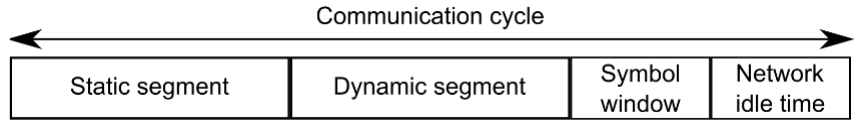
\includegraphics[width=\linewidth]{figures/Lecture2/flexraycommunicationcycle.png}
    \label{fig:placeholder}
\end{figure}
\subsection*{Communication Cycle Duration}

\begin{itemize}
    \item Typical FlexRay communication cycle durations are:
    \[
    2.5\,\text{ms},\ 5\,\text{ms},\ \text{or}\ 10\,\text{ms}
    \]
    
    \item The selected cycle duration depends on the
    \textbf{shortest periodic timing requirement} in the system.
    
    \item Real-time automotive applications require predictable and periodic communication.
\end{itemize}

\section{Static Segment}

\begin{itemize}
    \item The \textbf{static segment} is always transmitted first in the communication cycle.
    
    \item Communication in the static segment is based on
    \textbf{Time Division Multiple Access (TDMA)}.
    
    \item Each ECU is assigned predefined time slots.
    
    \item Each static frame is transmitted in exactly one static slot.
    
    \item All static slots have identical duration:
    \[
    \texttt{gdStaticSlot}
    \]
    
    \item Since transmission times are fixed and known in advance,
    deterministic communication is guaranteed.
    
    \item An application or task may be assigned
    \textbf{multiple static slots} within the same communication cycle.
    
    \item This is useful when:
    \begin{itemize}
        \item the application produces large amounts of data,
    \end{itemize}
    \item For example, a braking controller may transmit:
    \begin{itemize}
        \item wheel sensor data in one slot,
        \item control commands in another slot,
        \item diagnostic information in additional slots.
    \end{itemize}
\end{itemize}

\subsection*{Example Application: ABS}

\begin{itemize}
    \item A typical static-segment application is an
    \textbf{Anti-lock Braking System (ABS)}.
    
    \item Wheel speed sensors must be sampled continuously and periodically.
    
    \item Deterministic timing ensures:
    \begin{itemize}
        \item predictable sensor updates,
        \item synchronized control actions,
        \item reliable braking performance.
    \end{itemize}
\end{itemize}

\section{Dynamic segment (How Minislots Work)}

\begin{itemize}
    \item The dynamic segment is divided into equal-duration
    \textbf{minislots}.
    
    \item Each minislot represents a \textbf{transmission opportunity}, not a fixed assignment to a specific ECU or frame.
    
    \item At each minislot boundary:
    \begin{itemize}
        \item all nodes with pending messages are considered,
        \item the message with the \textbf{highest priority (lowest Frame ID)} is selected.
    \end{itemize}
    
    \item If no node has data to transmit:
    \begin{itemize}
        \item the minislot expires immediately,
        \item the system proceeds to the next minislot.
    \end{itemize}
    
    \item If a node does transmit:
    \begin{itemize}
        \item it starts sending a full frame,
        \item transmission continues until the frame is complete,
        \item minislot progression is effectively paused during transmission.
    \end{itemize}
\end{itemize}
\begin{mdframed}[backgroundcolor=lightgray, linewidth=0pt, innertopmargin=8pt,
innerbottommargin=8pt]
\textbf{Key Idea}
\begin{itemize}
    \item A minislot is best understood as a repeated question:
    
    \begin{quote}
    \textit{“Which highest-priority message is ready to transmit right now?”}
    \end{quote}
    
    \item It is \textbf{not the transmission duration itself}, but the decision point for access.
\end{itemize}
\end{mdframed}
\subsection*{Typical Applications}

\begin{itemize}
    \item The dynamic segment is commonly used for
    \textbf{event-based applications}.
    
    \item Example:
    \begin{itemize}
        \item Turn signals,
        \item driver button presses,
        \item diagnostic events,
        \item status notifications.
    \end{itemize}
    
    \item These events occur only when triggered by the user or system.
\end{itemize}

\section*{Symbol Window}

\begin{itemize}
    \item After the dynamic segment, FlexRay provides a
    \textbf{symbol window}.
    
    \item The symbol window is used to transmit special bit patterns.
    
    \item Typical uses include:
    \begin{itemize}
        \item waking up sleeping nodes,
        \item network management,
        \item synchronization-related signaling.
    \end{itemize}
\end{itemize}

\section*{Network Idle Time (NIT)}

\begin{itemize}
    \item The communication cycle ends with
    \textbf{Network Idle Time (NIT)}.
    
    \item During this interval:
    \begin{itemize}
        \item no normal frame transmission occurs,
        \item nodes perform clock synchronization,
        \item timing corrections are applied.
    \end{itemize}
\end{itemize}
\begin{mdframed}[backgroundcolor=lightgray, linewidth=0pt, innertopmargin=8pt,
innerbottommargin=8pt]
\textbf{Key Takeaway:}
 NIT is essential for maintaining deterministic timing across all ECUs.
\end{mdframed}

\section{Communication Cycle: FlexRay vs. CAN}
\begin{mdframed}[backgroundcolor=lightgray, linewidth=0pt, innertopmargin=8pt,
innerbottommargin=8pt]
\begin{itemize}
    \item \textbf{CAN}
    \begin{itemize}
        \item No global communication cycle.
        \item Purely event-driven communication.
        \item Uses bitwise arbitration based on message priority.
    \end{itemize}

    \item \textbf{FlexRay}
    \begin{itemize}
        \item Uses a fixed communication cycle.
        \item Combines:
        \begin{itemize}
            \item static (time-triggered) segment,
            \item dynamic (event-triggered) segment.
        \end{itemize}
    \end{itemize}

    \item \textbf{Dynamic Segment vs CAN}
    \begin{itemize}
        \item Both are event-driven and priority-based.
        \item CAN resolves conflicts during transmission.
        \item FlexRay resolves access at minislot boundaries within a scheduled cycle.
    \end{itemize}
\end{itemize}
\end{mdframed}



\section{Timing Hierarchy What is Shared vs What is Local?}
\begin{figure}[H]
    \centering
    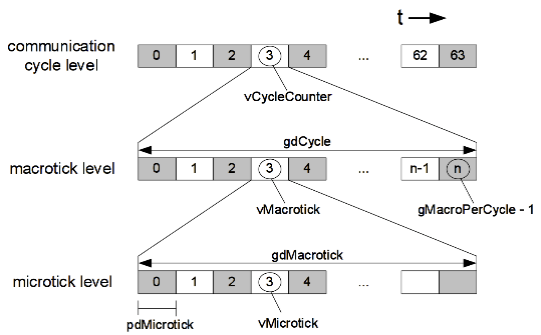
\includegraphics[width=0.7\linewidth]{figures/Lecture2/flexrayTimingHier.png}
    \label{fig:placeholder}
\end{figure}
\begin{figure}[H]
    \centering
    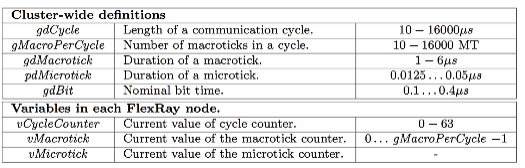
\includegraphics[width=0.7\linewidth]{figures/Lecture2/timingsFlex.png}
    \label{fig:placeholder}
\end{figure}
\subsubsection*{Shared (global across all nodes)}
\begin{itemize}
    \item Communication cycle length
    \item Number of macroticks per cycle
    \item Cycle counter (cycle 0, 1, 2, \dots)
\end{itemize}

\textbf{This is identical for every ECU.}

\textbf{So yes:}
\begin{itemize}
    \item all nodes are always in the same cycle,
    \item and at the same macrotick position.
\end{itemize}

\subsubsection*{Local (inside each ECU/controller)}
\begin{itemize}
    \item Microticks are local hardware clock ticks.
    \item Each ECU has its own oscillator + hardware timer.
    \item Microtick speed can differ slightly between controllers.
\end{itemize}

\textbf{BUT:}

\begin{itemize}
    \item FlexRay continuously synchronizes all nodes so that macroticks stay aligned globally.
\end{itemize}

\begin{mdframed}[backgroundcolor=lightgray, linewidth=0pt, innertopmargin=8pt,
innerbottommargin=8pt]
\textbf{Key takeaway:}

\begin{itemize}
    \item FlexRay does NOT require microticks to match across ECUs.
    \item Instead, each ECU uses its local microtick clock (hardware-dependent) to derive timing.
    \item It Requires All ECUs must agree on macrotick timing
    \item macrotick duration (real time) is synchronized across the network,
\end{itemize}
\end{mdframed}

\section{Communication Cycle Structure (Start Times)}
\begin{figure}[H]
    \centering
    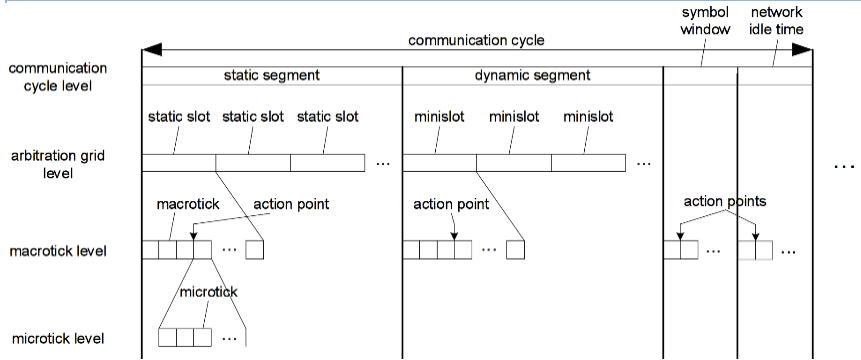
\includegraphics[width=\linewidth]{figures/Lecture2/actionpoint.png}
    \label{fig:placeholder}
\end{figure}
\section{Static Segment: Action Point Concept}

\subsubsection*{Static Slot Behavior}
\begin{itemize}
    \item Each frame corresponds to exactly one static slot.
    \item Every slot has equal length ($gdStaticSlot$).
    \item Slots are strictly scheduled using Time Division Multiple Access (TDMA).
\end{itemize}

\subsubsection*{“Action Point” Meaning}

\textbf{“Transmission must start at an action point instant”} means:

\begin{itemize}
    \item Each slot has a precise start boundary.
    \item This boundary is aligned with the global macrotick clock.
    \item ECUs are only allowed to start transmission exactly at this instant.
\end{itemize}
\begin{mdframed}[backgroundcolor=lightgray, linewidth=0pt, innertopmargin=8pt,
innerbottommargin=8pt]
\textbf{Key Idea}
\begin{itemize}
    \item Static TDMA in FlexRay is not just “time slots”, but hard real-time slots with fixed start instants.
    \item start times are globally synchronized,
\end{itemize}
\end{mdframed}


\section{Dynamic Segment Timing (FlexRay)}
\begin{itemize}
    \item Macroticks are still used as the global timing base.
\end{itemize}

\textbf{What still uses macroticks}
\begin{itemize}
    \item Time is structured using macroticks.
    \item Minislots are aligned to this global time base.
    \item The global clock remains synchronized across all ECUs.
\end{itemize}

\textbf{ What is NOT fixed anymore}
\begin{itemize}
    \item There is no fixed ``your slot starts at macrotick X'' assignment.
    \item There is no pre-assigned transmission start instant per ECU.
\end{itemize}

\subsubsection*{So what actually happens?}

\begin{itemize}
    \item The system continuously advances through minislots.
    \item Each minislot is aligned to the global time base (macroticks underneath).
    \item At each minislot boundary:
    \begin{itemize}
        \item arbitration takes place,
        \item the highest priority ready frame may start transmission.
    \end{itemize}
\end{itemize}



\section{Dynamic Minislotting}
\begin{figure}[H]
    \centering
    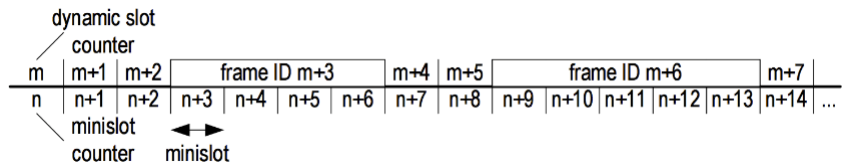
\includegraphics[width=\linewidth]{figures/Lecture2/minislotting.png}
    \label{fig:placeholder}
\end{figure}
\begin{itemize}
    \item Each node has one or more \textbf{frames with unique Frame IDs}, which also define priority.
    
    \item A global \textbf{dynamic slot counter} runs through the dynamic segment.
    
    \item A node is allowed to start transmission when:
    \[
    \text{slot counter} = \text{Frame ID}
    \]
    
    \item While a frame is transmitting:
    \begin{itemize}
        \item the slot counter is frozen,
        \item transmission continues over multiple minislots until the frame is complete.
    \end{itemize}
    
    \item If no transmission occurs in a minislot:
    \begin{itemize}
        \item the slot counter simply advances,
        \item and the minislot is consumed without data transmission.
    \end{itemize}
\end{itemize}

\subsubsection*{Cycle Structure}

\begin{itemize}
    \item The number of minislots per cycle is fixed:
    \[
    gNumberOfMinislots
    \]
    
    \item After all minislots are used, the cycle ends and the slot counter resets.
    
    \item Depending on traffic load:
    \begin{itemize}
        \item more/longer frames cause the slot counter to progress more slowly,
        \item fewer transmissions allow it to reach higher values.
        \item This also means that you may never reach the higher count of the minislots, if larger/many transmission is done for higher priority frames
    \end{itemize}
\end{itemize}

\subsubsection*{Transmission Limit}

\begin{itemize}
    \item Each node has a parameter:
    \[
    pLatestTx
    \]
    
    \item This defines the last minislot where a frame can still start transmission.
    
    \item If the slot counter exceeds $pLatestTx$:
    \begin{itemize}
        \item the node is no longer allowed to transmit in this cycle,
        \item pending frames are postponed to the next communication cycle.
    \end{itemize}
\end{itemize}

\section{Dynamic Minislotting: FlexRay vs. CAN}

\begin{itemize}
    \item \textbf{How is it compared to CAN?}
    
    \item \textbf{Similarities:}
    \begin{itemize}
        \item Both use \textbf{prioritized access} based on message identifiers.
        \item Higher priority messages are transmitted first.
        \item Lower priority messages may be delayed or postponed under heavy bus load.
    \end{itemize}
    
    \item \textbf{Differences:}
    \begin{itemize}
        \item In CAN, bus arbitration happens during transmission (bitwise arbitration).
        \item In FlexRay dynamic minislotting, access is decided at discrete minislot boundaries.
        \item Even if no transmission occurs in a minislot, the system still consumes that minislot time.
    \end{itemize}
    
    \item \textbf{Key Insight:}
    \begin{itemize}
        \item FlexRay maintains a fixed time structure, so every minislot always advances the global schedule.
        \item This guarantees deterministic timing, even when the bus is idle.
    \end{itemize}
\end{itemize}
\section{Flexray Frame Layout}
\begin{figure}[H]
    \centering
    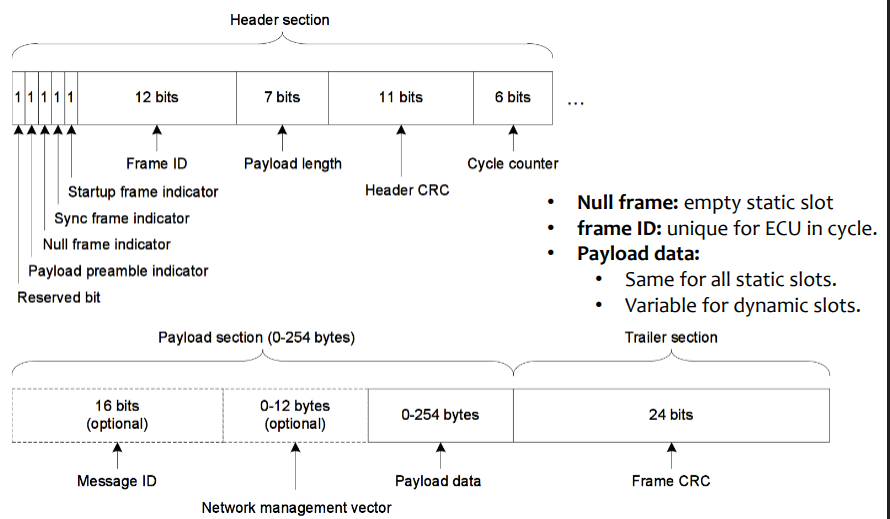
\includegraphics[width=\linewidth]{figures/Lecture2/flexray FrameLayout.png}
    \label{fig:placeholder}
\end{figure}


\section{Frame Layout: FlexRay vs. CAN and Ethernet}

\subsection*{FlexRay vs. CAN}

\begin{itemize}
    \item FlexRay uses a \textbf{12-bit Frame ID}, while CAN uses an \textbf{11-bit identifier}.
    
    \item In both CAN and FlexRay:
    \begin{itemize}
        \item the ID represents the message content (not a destination address),
        \item lower ID means higher priority.
    \end{itemize}
    
    \item However, there is a key difference:
    \begin{itemize}
        \item In \textbf{CAN}, arbitration happens during transmission using bitwise arbitration on the bus.
        \item In \textbf{FlexRay}, priority is used in a scheduled way (especially in the dynamic segment via minislotting).
    \end{itemize}
    
    \item CAN payload is limited to \textbf{0--8 bytes}, while FlexRay supports larger payloads.
    
    \item In FlexRay, payload and timing structure differ between segments:
    \begin{itemize}
        \item static segment: fixed length frames,
        \item dynamic segment: variable-length frames.
    \end{itemize}
\end{itemize}

\subsection*{FlexRay vs. Ethernet}

\begin{itemize}
    \item Ethernet supports variable frame sizes (typically \textbf{0--1500 bytes} MTU).
    
    \item Ethernet uses a \textbf{destination address} for communication instead of a Frame ID.
    
    \item Unlike FlexRay and CAN, Ethernet is packet-switched and not inherently time-deterministic.
\end{itemize}



\section{Performance Aspects of Flexray}

\subsection*{Throughput}

\begin{itemize}
    \item For sensor data, throughput is often not the main design priority.
    
    \item In in-car networks (e.g., software updates), high throughput is important.
    
    \item \textbf{Static segment:}
    \begin{itemize}
        \item Throughput depends on cycle time and payload length.
        \item All slots have equal length, so increasing payload typically increases cycle time (for a fixed number of nodes).
        \item Higher throughput for one ECU can be achieved by assigning multiple static slots.
    \end{itemize}
    
    \item \textbf{Dynamic segment:}
    \begin{itemize}
        \item Higher throughput can be achieved using larger payloads.
        \item However, long frames may block the bus longer and increase delay for other messages.
    \end{itemize}
\end{itemize}

\subsection*{Delay and Jitter}

\begin{itemize}
    \item \textbf{Static segment:}
    \begin{itemize}
        \item Fully deterministic timing.
        \item Maximum delay is bounded by the next communication cycle.
    \end{itemize}
    
    \item \textbf{Dynamic segment:}
    \begin{itemize}
        \item Messages may be postponed to later cycles.
        \item Minislot-based access can lead to varying transmission timing.
        \item This results in higher jitter compared to the static segment.
    \end{itemize}
\end{itemize}

\subsection*{Redundancy}

\begin{itemize}
    \item \textbf{Spatial redundancy:}
    \begin{itemize}
        \item Dual-channel configuration reduces risk of communication failure.
        \item Protects against electrical interference or cable faults.
    \end{itemize}
    
    \item \textbf{Temporal redundancy:}
    \begin{itemize}
        \item Messages are transmitted multiple times.
        \item For example, in every cycle or via multiple slot assignments.
    \end{itemize}
\end{itemize}

\subsection*{Loss Handling (CAN vs. FlexRay)}

\begin{itemize}
    \item \textbf{CAN:}
    \begin{itemize}
        \item Supports automatic retransmission of frames if errors are detected or no acknowledgment is received.
        \item The transmitter will retry until the message is successfully delivered or an error limit is reached.
        \item This improves reliability but does not guarantee a fixed delivery time.
    \end{itemize}
    
    \item \textbf{FlexRay:}
    \begin{itemize}
        \item No automatic retransmission is performed.
        \item Lost messages must be handled by the application layer.
        \item This design supports deterministic timing.
    \end{itemize}
\end{itemize}
\section{Dynamic Segment State Machine (Markov Chain View)}
\begin{figure}[H]
    \centering
    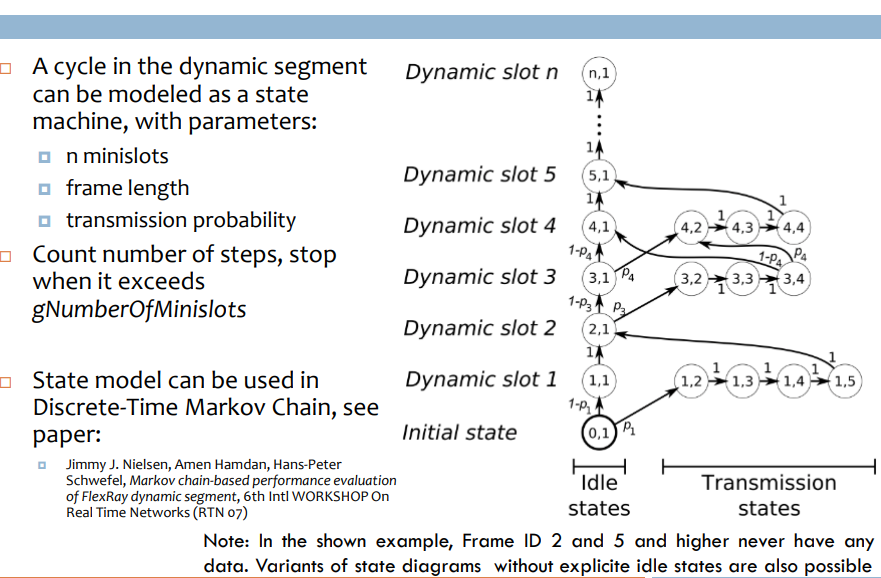
\includegraphics[width=\linewidth]{figures/Lecture2/markovDynamic.png}
    \label{fig:placeholder}
\end{figure}
\begin{itemize}
    \item The system state is defined by parameters such as:
    \begin{itemize}
        \item number of remaining minislots ($n$),
        \item frame length,
        \item probability that a node has data to transmit.
    \end{itemize}
    
    \item A cycle evolves step-by-step through minislots, and stops when:
    \[
    \text{slot counter} > gNumberOfMinislots
    \]
    
    \item Depending on which frames are ready for transmission, the system transitions between different states.
    
    \item This behavior can be modeled as a \textbf{Discrete-Time Markov Chain (DTMC)}, where:
    \begin{itemize}
        \item each state represents a minislot configuration,
        \item transitions depend on transmission probability and frame availability.
    \end{itemize}
    
    \item The model captures that:
    \begin{itemize}
        \item some Frame IDs may never be active (idle states),
        \item different cycles may experience different numbers of transmissions,
        \item the dynamic segment length in terms of activity can vary statistically.
    \end{itemize}
\end{itemize}


\section*{Discrete-Time Markov Chain Model (Dynamic Segment)}

\textbf{Purpose:}
The dynamic segment of FlexRay can be approximated using a Discrete-Time Markov Chain (DTMC) to evaluate performance metrics such as delay and displacement probability.

\subsubsection*{Model Assumptions}

\begin{itemize}
    \item \textbf{Constant frame length per Frame ID}
    \begin{itemize}
        \item Each Frame ID is assumed to have a fixed transmission time.
        \item This simplifies the model by removing variable payload effects.
    \end{itemize}
    
    \item \textbf{i.i.d. frame arrivals}
    \begin{itemize}
        \item Each frame arrives independently with probability $p_i$.
        \item No correlation between arrivals in different minislots or cycles.
        \item This preserves the Markov property.
    \end{itemize}
\end{itemize}

\subsubsection*{System Evolution}

\begin{itemize}
    \item The dynamic segment contains:
    \[
    gNumberOfMinislots
    \]
    
    \item Each minislot represents one discrete time step in the Markov chain.
    
    \item The system evolves over $k = gNumberOfMinislots$ steps per cycle.
\end{itemize}

\subsubsection*{Displacement Probability}

\begin{itemize}
    \item Due to limited minislots, not all frames may be transmitted within a cycle.
    
    \item Frames that are not transmitted are \textbf{displaced to the next cycle}.
    
    \item The displacement probability is obtained from the state probabilities of the DTMC after $k$ steps.
\end{itemize}
\begin{mdframed}[backgroundcolor=lightgray, linewidth=0pt, innertopmargin=8pt,
innerbottommargin=8pt]
\textbf{Key Idea:}
\begin{itemize}
    \item The model approximates how often traffic cannot be served within a cycle due to minislot limitations.
    \item This provides a probabilistic measure of delay in the dynamic segment.
\end{itemize}
\end{mdframed}
\subsubsection*{State Evolution}

\[
\pi(k) = \pi(0) P^{k}
\]
probability distribution after k steps (end of dynamic segment)
\begin{itemize}
    \item $\pi(k)$: State probability vector after $k$ steps (minislots).
    
    \item $\pi(0)$: Initial state distribution of the system.
    
    \item $P$: Transition probability matrix of the Markov chain.
    
    \item $k$: Number of minislots in one dynamic segment cycle.
\end{itemize}
\subsubsection*{Displacement Probability}

\[
P(\text{s is displaced}) =
\sum_{b=2}^{l_s} \pi(k)_{s,b}
\;+\;
p_s \cdot \sum_{a=1}^{s-1}
\left(
\sum_{b=1}^{l_{max}+1} \pi(k)_{a,b}
\right)
\]
Probability that Frame ID s does NOT get transmitted in the current cycle (i.e., is delayed to next cycle)
\begin{itemize}
    \item $P(\text{s is displaced})$: Probability that a frame with Frame ID $s$ is not transmitted in the current cycle and is delayed to the next cycle.
    
    \item $l_s$: Frame length (in minislots) for Frame ID $s$.
    
    \item $l_{max}$: Maximum possible frame length (in minislots).
    
    \item $p_s$: Arrival probability of a frame with Frame ID $s$.
    
    \item $\pi(k)_{a,b}$: Probability of being in state $(a,b)$ after $k$ steps, where:
    \begin{itemize}
        \item $a$ represents the Frame ID / slot state,
        \item $b$ represents progress within a frame or minislot position.
    \end{itemize}
\end{itemize}